% !TEX encoding = UTF-8 Unicode
%%%%%%%%%%%%%%%%%%%%%%%%%%%%%%%%%%%%%%%%%
% Beamer Presentation
% LaTeX Template
% Version 1.0 (10/11/12)
%
% This template has been downloaded from:
% http://www.LaTeXTemplates.com
%
% License:
% CC BY-NC-SA 3.0 (http://creativecommons.org/licenses/by-nc-sa/3.0/)
%
%%%%%%%%%%%%%%%%%%%%%%%%%%%%%%%%%%%%%%%%%

%----------------------------------------------------------------------------------------
%	PACKAGES AND THEMES
%----------------------------------------------------------------------------------------

\documentclass{beamer}

\mode<presentation> {

% The Beamer class comes with a number of default slide themes
% which change the colors and layouts of slides. Below this is a list
% of all the themes, uncomment each in turn to see what they look like.

%\usetheme{default}
%\usetheme{AnnArbor}
%\usetheme{Antibes}
%\usetheme{Bergen}
%\usetheme{Berkeley}
%\usetheme{Berlin}
%\usetheme{Boadilla}
%\usetheme{CambridgeUS}
%\usetheme{Copenhagen}
%\usetheme{Darmstadt}
%\usetheme{Dresden}
%\usetheme{Frankfurt}
%\usetheme{Goettingen}
%\usetheme{Hannover}
%\usetheme{Ilmenau}
%\usetheme{JuanLesPins}
%\usetheme{Luebeck}
%\usetheme{Madrid}
%\usetheme{Malmoe}
%\usetheme{Marburg}
%\usetheme{Montpellier}
%\usetheme{PaloAlto}
%\usetheme{Pittsburgh}
%\usetheme{Rochester}
\usetheme{Singapore}
%\usetheme{Szeged}
%\usetheme{Warsaw}

% As well as themes, the Beamer class has a number of color themes
% for any slide theme. Uncomment each of these in turn to see how it
% changes the colors of your current slide theme.

%\usecolortheme{albatross}
%\usecolortheme{beaver}
%\usecolortheme{beetle}
%\usecolortheme{crane}
%\usecolortheme{dolphin}
%\usecolortheme{dove}
%\usecolortheme{fly}
%\usecolortheme{lily}
%\usecolortheme{orchid}
%\usecolortheme{rose}
%\usecolortheme{seagull}
%\usecolortheme{seahorse}
%\usecolortheme{whale}
%\usecolortheme{wolverine}

%\setbeamertemplate{footline} % To remove the footer line in all slides uncomment this line
%\setbeamertemplate{footline}[page number] % To replace the footer line in all slides with a simple slide count uncomment this line

%\setbeamertemplate{navigation symbols}{} % To remove the navigation symbols from the bottom of all slides uncomment this line
}

\usepackage{graphicx} % Allows including images
\usepackage{booktabs} % Allows the use of \toprule, \midrule and \bottomrule in tables
\usepackage{xeCJK}
\setCJKmainfont{SourceHanSerif-Regular}
\usepackage{color}
\usepackage{listings}
\lstset{numbers=left}
\usepackage{fancyvrb}%use Verbatim-the extended verbatim
\usepackage{tikz}


%----------------------------------------------------------------------------------------
%	TITLE PAGE
%----------------------------------------------------------------------------------------

\title[Django]{python} % The short title appears at the bottom of every slide, the full title is only on the title page
\subtitle{控制结构}
\author{} % Your name
\institute[计算机科学与技术学院] % Your institution as it will appear on the bottom of every slide, may be shorthand to save space
{
贵州大学 \\ % Your institution for the title page
\medskip
\textit{hnzhang1@gzu.edu.cn} % Your email address
}
\date{\today} % Date, can be changed to a custom date

\begin{document}

\begin{frame}
\titlepage % Print the title page as the first slide
\end{frame}
\begin{frame}{Overview}
\tableofcontents
\end{frame}
\section{关系和逻辑运算符}
\begin{frame}{条件}
控制结构包括:判断和循环。为了作出判断或控制循环,必须指定条件来做依据。

条件(也叫布尔表达式)是一种包含了关系运算符($>$、$>=$、$=$等)和(或)逻辑运算符($and$、$or$、$not$)的表达式。

条件的结果为:True或False。
\end{frame}
\begin{frame}[fragile]{ASCII}
在应用关系运算符进行比较字符时的依据是这些字符的ASCII\footnote{ASCII(American Standard Code for Information Interchange,美国信息交换标准代码)是基于拉丁字母的一套电脑编码系统。}值。
\begin{block}{}
\begin{Verbatim}[numbers=left,frame=single,rulecolor=\color{red}]
ord(c, /)
    Return the ASCII value for a one-character string.
chr(i, /)
    Return a  string of the ASCII, …
>>> print("ord('A')",ord('A'),"; ord('Z')",ord('Z'),\
... "| ord('a')",ord('a'),"; ord('z')",ord('z'))
ord('A') 65 ; ord('Z') 90 | ord('a') 97 ; ord('z') 122
>>> print("chr(48)",chr(48),"; chr(57)",chr(57),\
... "| chr(169)",chr(169),"; chr(248)",chr(248))
chr(48) 0 ; chr(57) 9 | chr(169) © ; chr(248) ø
\end{Verbatim}
\end{block}

\end{frame}
\section{判断结构}
\section{循环结构}
\subsection{while循环}
\subsection{for循环}



\begin{frame}[fragile]{不可变和可变对象内存示意}
\begin{columns}[c]  %开始进入分栏环境,居中设置
\column{3.2cm}  %第一栏(左栏)宽度为8cm
\begin{block}{}
\begin{Verbatim}[numbers=left,frame=single,rulecolor=\color{red}]
>>> l=[1,2]
>>> i=3
>>> s="python"
>>> t=(4,5)
>>> l.append(3)
>>> i+=1
>>> s=s.upper()
>>> t=t[1:]
\end{Verbatim}
\end{block}
\column{3cm}  %第二栏(右栏)宽度为3cm
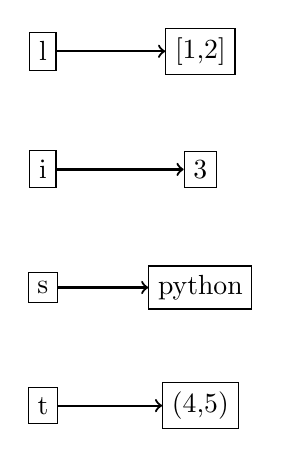
\begin{tikzpicture}
%\draw [thick,red,dashed,above] (0,0) rectangle (3,5) node{host A};
\node [draw,rectangle] (l) at(0,4.5){l};
\node [draw,rectangle] (lv) at(2,4.5){[1,2]};

\node [draw,rectangle] (i) at(0,3){i};
\node [draw,rectangle] (iv) at(2,3){3};

\node [draw,rectangle] (s) at(0,1.5){s};
\node [draw,rectangle] (sv) at(2,1.5){python};

\node [draw,rectangle] (t) at(0,0){t};
\node [draw,rectangle] (tv) at(2,0){(4,5)};
%\node [draw,rectangle] (o) at(4,0){output};
%\draw [thick,blue,dashed,above] (5,0) rectangle (8,5)node{host B};
%\node [draw,rectangle] (pb1) at(6.5,3){process B1};
%\node [draw,rectangle] (pb2) at(6.5,2){...};
\draw[thick,->](l) to[out=0,in=180] (lv);
\draw[thick,->](i) to[out=0,in=180] (iv);
\draw[thick,->](s) to[out=0,in=180] (sv);
\draw[thick,->](t) to[out=0,in=180] (tv);
%\draw[thick,->](p) to[out=0,in=180] (o);


\end{tikzpicture}

\column{3cm}  %第二栏(右栏)宽度为3cm
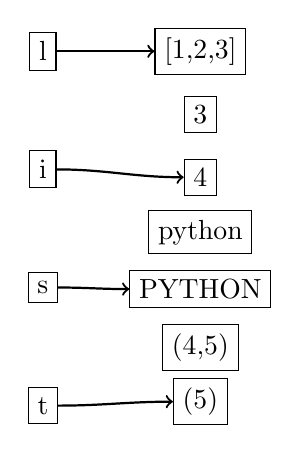
\begin{tikzpicture}
%\draw [thick,red,dashed,above] (0,0) rectangle (3,5) node{host A};

\node [draw,rectangle] (l) at(0,4.5){l};
\node [draw,rectangle] (lv) at(2,4.5){[1,2,3]};

\node [draw,rectangle] (i) at(0,3){i};
\node [draw,rectangle] (ivv) at(2,3.7){3};
\node [draw,rectangle] (iv) at(2,2.9){4};

\node [draw,rectangle] (s) at(0,1.5){s};
\node [draw,rectangle] (svv) at(2,2.2){python};
\node [draw,rectangle] (sv) at(2,1.48){PYTHON};

\node [draw,rectangle] (t) at(0,0){t};
\node [draw,rectangle] (tvv) at(2,0.74){(4,5)};
\node [draw,rectangle] (tv) at(2,0.05){(5)};
%\node [draw,rectangle] (o) at(4,0){output};
%\draw [thick,blue,dashed,above] (5,0) rectangle (8,5)node{host B};
%\node [draw,rectangle] (pb1) at(6.5,3){process B1};
%\node [draw,rectangle] (pb2) at(6.5,2){...};
\draw[thick,->](l) to[out=0,in=180] (lv);
\draw[thick,->](i) to[out=0,in=180] (iv);
\draw[thick,->](s) to[out=0,in=180] (sv);
\draw[thick,->](t) to[out=0,in=180] (tv);
\end{tikzpicture}
\end{columns}  %分栏环境结束


\end{frame}

%----------------------------------------------------------------------------------------
%	PRESENTATION SLIDES
%----------------------------------------------------------------------------------------
\section{homework}
\begin{frame}{Homework}
\begin{enumerate}
\item
计算$x^{y}$.(x, y的值使用input获取)
%\item
%找零钱。输入收费金额和客户所付的钱,给出需要怎么找零。要求找零的钱币张数最少。(即需要多少1元的,多少2元的,多少5元的等)
\end{enumerate}
\end{frame}
\section{Q\&A}
\begin{frame}
\center{\Huge{Q\&A}}
\end{frame}


%How do I uninstall?
%
%	1.	Remove /Applications/Wireshark.app
%	2.	Remove /Library/Application Support/Wireshark
%	3.	Remove the wrapper scripts from /usr/local/bin
%	4.	Unload the org.wireshark.ChmodBPF.plist launchd job
%	5.	Remove /Library/LaunchDaemons/org.wireshark.ChmodBPF.plist
%	6.	Remove the access_bpf group.
%	7.	Remove /etc/paths.d/Wireshark
%	8.	Remove /etc/manpaths.d/Wireshark
\end{document} 

